\tikzset{
  every picture/.style={font=\scriptsize},
}
\definecolor{dsflash}{HTML}{4E79A7}
\definecolor{dspro}{HTML}{F28E2B}
\definecolor{grokc}{HTML}{59A14F}
\definecolor{kimic}{HTML}{E15759}
\definecolor{gptc}{HTML}{B07AA1}
\definecolor{gridgray}{HTML}{D9D9D9}
\definecolor{riskred}{HTML}{B2182B}
\definecolor{riskorange}{HTML}{EF8A62}
\definecolor{riskorangeone}{HTML}{FDAE61}
\definecolor{riskyellow}{HTML}{FDDC8B}
\definecolor{riskneutral}{HTML}{FFFFBF}
\definecolor{riskgreenone}{HTML}{D9EF8B}
\definecolor{riskgreentwo}{HTML}{A6D96A}
\definecolor{riskgreenthree}{HTML}{66BD63}
\definecolor{riskgreenfour}{HTML}{1A9850}

\begin{tikzpicture}
\begin{axis}[
  width=\linewidth,
  height=0.27\textheight,
  tick label style={font=\tiny},
  label style={font=\scriptsize},
  legend style={font=\tiny, draw=none, fill=none},
  ymajorgrids=true,
  grid style={gridgray},
  ymin=0,
  ymax=10.5,
  ylabel={$N_{\mathrm{safe}}$},
  width=0.58\linewidth, height=0.19\textheight, ybar, symbolic x coords={DeepSeek-V4-Flash,DeepSeek-V4-Pro}, xtick=data, xticklabel style={font=\tiny}, enlarge x limits=0.34, legend style={font=\tiny, draw=none, fill=white, fill opacity=0.9, text opacity=1, at={(0.98,0.98)}, anchor=north east},
]
\addplot[ybar, bar width=14pt, bar shift=-8pt, fill=dsflash, draw=none, error bars/.cd, y dir=both, y explicit, error bar style={black, thick}] coordinates {(DeepSeek-V4-Flash,4.357) +- (0,0.152) (DeepSeek-V4-Pro,3.867) +- (0,0.083)};
\addplot[ybar, bar width=14pt, bar shift=8pt, fill=dspro, draw=none, error bars/.cd, y dir=both, y explicit, error bar style={black, thick}] coordinates {(DeepSeek-V4-Flash,4.013) +- (0,0.013) (DeepSeek-V4-Pro,4.030) +- (0,0.012)};
\addplot[black, dashed, sharp plot, forget plot] coordinates {(DeepSeek-V4-Flash,4) (DeepSeek-V4-Pro,4)};
\legend{disabled, enabled}
\end{axis}
\end{tikzpicture}
